\documentclass[a4paper,12pt]{article}
\usepackage[utf8]{inputenc}
\usepackage[T2A]{fontenc}
\usepackage[russian, english]{babel}
\usepackage[left=2cm, right=2cm, top=2cm, bottom=2cm]{geometry}
\usepackage{graphicx}
\usepackage{float}
\usepackage{wrapfig}
\usepackage{tikz}
\usepackage{amsmath, amsfonts, amssymb}
\usepackage{hyperref}
\hypersetup{pdfborder=0 0 0, pdfstartview=FitH, linkcolor=blue, urlcolor=blue, colorlinks=true}
\usepackage{fancybox, fancyhdr}
\pagestyle{fancy}

\usepackage{xcolor}
\definecolor{urlcolor}{HTML}{3454D1}
\definecolor{linkcolor}{HTML}{3454D1}

\usepackage{listings}
\lstdefinestyle{codestyle}{
    backgroundcolor=\color{gray!10},
    commentstyle=\color{green!50!black},
    keywordstyle=\color{blue!80!black},
    stringstyle=\color{red!50!black},
    numberstyle=\tiny\color{gray},
    basicstyle=\ttfamily\footnotesize,
    breaklines=true,
    captionpos=b,
    numbers=left,
    numbersep=5pt,
    showstringspaces=false,
    tabsize=2
}
\lstset{style=codestyle}

\usepackage{mdframed}
\newmdenv[
  leftmargin = 0.5em,
  skipabove = 0.5em,
  skipbelow = 0.5em,
  linewidth = 1pt,
  rightline = false,
  topline = false,
  bottomline = false
]{quotebox}

\begin{document}

% Титульный лист
\begin{titlepage}
    \centering
    {\large Федеральное государственное автономное образовательное учреждение\par}
    {\large высшего образования\par}
    {\bfseries САНКТ-ПЕТЕРБУРГСКИЙ НАЦИОНАЛЬНЫЙ ИССЛЕДОВАТЕЛЬСКИЙ УНИВЕРСИТЕТ ИТМО\par}
    {\bfseries Факультет систем управления и робототехники\par}
    \vfill
    {\Large \bfseries Лабораторная работа №1\par}
    {\Large \bfseries Задачи №1322, 1444, 1604\par}
    \vfill
    
    \begin{flushright}
        Студент: Сайфуллин Д.Р. \\
        Поток: АиСД R23 1.3 \\
        Преподаватель: Тропченко А.А.
    \end{flushright}
    \vfill
    Санкт-Петербург \\
    2025 г.
\end{titlepage}

\section*{Задача №1322. Шпион}
Спецслужбы обнаружили действующего иностранного агента. Шпиона то есть. Установили наблюдение и выяснили, что каждую неделю он через Интернет посылает кому-то странные нечитаемые тексты. Чтобы выяснить, к какой информации получил доступ шпион, требуется расшифровать информацию. Сотрудники спецслужб проникли в квартиру разведчика, изучили шифрующее устройство и выяснили принцип его работы.\\[0.5em]
На вход устройства подается строка текста S1 = s1s2...sN. Получив ее, устройство строит все циклические перестановки этой строки, то есть S2 = s2s3...sNs1, ..., SN = sNs1s2...sN-1. Затем множество строк S1, S2, ..., SN сортируется лексикографически по возрастанию. И в этом порядке строчки выписываются в столбец, одна под другой. Получается таблица размером N × N. В какой-то строке K этой таблицы находится исходное слово. Номер этой строки вместе с последним столбцом устройство и выдает на выход.\\[0.5em]
Например, если исходное слово S1 = abracadabra, то таблица имеет такой вид:
\begin{itemize}
    \item aabracadabr = S11
    \item abraabracad = S8
    \item abracadabra = S1
    \item acadabraabr = S4
    \item adabraabrac = S6
    \item braabracada = S9
    \item bracadabraa = S2
    \item cadabraabra = S5
    \item dabraabraca = S7
    \item raabracadab = S10
    \item racadabraab = S3
\end{itemize}
И результатом работы устройства является число 3 и строка rdarcaaaabb.\\[0.5em]
Это все, что известно про шифрующее устройство. А вот дешифрующего устройства не нашли. Но поскольку заведомо известно, что декодировать информацию можно (а иначе зачем же ее передавать?), Вам предложили помочь в борьбе с хищениями секретов и придумать алгоритм для дешифровки сообщений. А заодно и реализовать дешифратор.\\[1em]
\textbf{Исходные данные:}
\begin{quotebox}
    В первой и второй строках находятся соответственно целое число и строка, возвращаемые шифратором. Длина строки и число не превосходят $10^5$. Строка содержит лишь следующие символы: a-z, A-Z, символ подчеркивания. Других символов в строке нет. Лексикографический порядок на множестве слов задается таким порядком символов:
    ABCDEFGHIJKLMNOPQRSTUVWXYZ\_abcdefghijklmnopqrstuvwxyz\\[0.5em]
    Символы здесь выписаны в порядке возрастания.
\end{quotebox}
\textbf{Результат:}
\begin{quotebox}
    Выведите декодированное сообщение в единственной строке.
\end{quotebox}
\subsection*{Рабочий код}
\begin{lstlisting}[language=python]
def decode_bwt(k, last_column):
    n = len(last_column)

    temp = sorted([(char, i) for i, char in enumerate(last_column)])

    result = []
    k -= 1
    for _ in range(n):
        result.append(temp[k][0])
        k = temp[k][1]

    return ''.join(result)


k = int(input().strip())
last_column = input().strip()

print(decode_bwt(k, last_column))
\end{lstlisting}
\subsection*{Объяснение алгоритма}
Этот код выполняет сортировку символов в строке и затем переставляет их в декодированном порядке. Алгоритм сначала создает список пар (символ, индекс) и сортирует их по лексикографическому порядку символов. Затем, используя второй элемент пары (индекс), происходит восстановление исходной строки, начиная с позиции $k-1$. В процессе декодирования символы извлекаются в порядке, определяемом отсортированными индексами, что позволяет воссоздать исходное сообщение.
\newpage
\section*{Задача №1444. Накормить элефпотама}
Гарри Поттер сдаёт экзамен по предмету «Уход за магическими существами». Его задание — накормить карликового элефпотама. Гарри помнит, что элефпотамы отличаются прямолинейностью и невозмутимостью. Они настолько прямолинейны, что ходят строго по прямой, и настолько невозмутимы, что заставить их идти можно, только если привлечь его внимание к чему-нибудь действительно вкусному. И главное, наткнувшись на цепочку своих собственных следов, элефпотам впадает в ступор и отказывается идти куда-либо. По словам Хагрида, элефпотамы обычно возвращаются домой, идя в обратную сторону по своим собственным следам. Поэтому они никогда не пересекают их, иначе могут заблудиться. Увидев свои следы, элефпотам детально вспоминает все свои перемещения от выхода из дома (поэтому-то они и ходят только по прямой и лишний раз не меняют направление — так легче запоминать). По этой информации элефпотам вычисляет, в какой стороне расположена его нора, после чего поворачивается и идет прямо к ней. Эти вычисления занимают у элефпотама некоторое (довольно большое) время. А то, что некоторые невежды принимают за ступор, на самом деле есть проявление выдающихся вычислительных способностей этого чудесного, хотя и медленно соображающего животного!\\[0.5em]
Любимое лакомство элефпотамов — слоновьи тыквы, именно они и растут на лужайке, где Гарри должен сдавать экзамен. Перед началом испытания Хагрид притащит животное к одной из тыкв. Скормив элефпотаму очередную тыкву, Гарри может направить его в сторону любой оставшейся тыквы. Чтобы сдать экзамен, надо провести элефпотама по лужайке так, чтобы тот съел как можно больше тыкв до того, как наткнется на свои следы.\\[1em]
\textbf{Исходные данные:}
\begin{quotebox}
    В первой строке входа находится число $N$ $(3 \leq N \leq 30000)$ — количество тыкв на лужайке. Тыквы пронумерованы от 1 до $N$, причем номер один присвоен той тыкве, у которой будет стоять элефпотам в начале экзамена. В следующих N строках даны координаты всех тыкв по порядку. Все координаты — целые числа от −1000 до 1000. Известно, что положения всех тыкв различны, и не существует прямой, проходящей сразу через все тыквы.
\end{quotebox}
\textbf{Результат:}
\begin{quotebox}
    В первой строке выхода вы должны вывести $K$ — максимальное количество тыкв, которое может съесть элефпотам. Далее по одному числу в строке выведите $K$ чисел — номера тыкв в порядке их обхода. Первым в этой последовательности всегда должно быть число 1.
\end{quotebox}
\subsection*{Рабочий код}
\begin{lstlisting}[language=python]
import math

def solve():
    n = int(input().strip())
    coords = [tuple(map(int, input().split())) for _ in range(n)]
    f_x, f_y = coords[0]
    pumpkins = [None] * n\
    pumpkins[0] = (0.0, -1.0, 1)

    for i in range(1, n):
        x, y = coords[i]
        length = (x - f_x)**2 + (y - f_y)**2
        degrees = math.degrees(math.atan2(y - f_y, x - f_x))
        if (y - f_y) < 0:
            degrees += 360.0
        pumpkins[i] = (length, degrees, i+1)
    pumpkins.sort(key=lambda p: (p[1], p[0]))

    start_point = 1
    for i in range(1, n - 1):
        if pumpkins[i+1][1] - pumpkins[i][1] > 179.999:
            start_point = i + 1
    print(n)
    print(1)

    for i in range(start_point, n):
        print(pumpkins[i][2])
    for i in range(1, start_point):
        print(pumpkins[i][2])

solve()

\end{lstlisting}
\subsection*{Объяснение алгоритма}
Первая точка выбирается как начало координат. По ходу считывания записывается угол каждой точки относительно оси Ox и расстояние до нового начала координат. После этого точки сортируются по углу и по расстоянию от начала координат, таким образом итоговая геометрия обхода будет похожа на розу ветров. После сортировки находится максимальный угол между направлениями на две соседние точки, чтобы найти начало обхода, исключающее пересечение с маршрутом 2 соседних точек. После всех операций выводится обход точек с точки входа.
\newpage
\section{Задача №1604. В Стране Дураков}
Главный бульдог-полицейский Страны Дураков решил ввести ограничение скоростного режима на автомобильной трассе, ведущей от Поля Чудес к пруду Черепахи Тортиллы. Для этого он заказал у Папы Карло $n$ знаков ограничения скорости. Папа Карло слабо разбирался в дорожном движении и поэтому изготовил знаки с разными ограничениями на скорость: 49 км/ч, 34 км/ч, 42 км/ч, и т.д. Всего получилось $k$ различных ограничений: $n_1$ знаков с одним ограничением, $n_2$ знаков со вторым ограничением, и т.д. $(n_1 + \dots + n_k = n)$.\\[0.5em]
Бульдог-полицейский ничуть не расстроился, получив такие знаки, напротив, он решил извлечь из этого экономическую выгоду. Дело в том, что по Правилам дорожного движения Страны Дураков ограничение на скорость действует вплоть до следующего знака. Если на знаке написано число 60, это означает, что участок от данного знака до следующего нужно проехать ровно со скоростью 60 километров в час — не больше и не меньше. Бульдог распорядился расставить знаки так, чтобы обогатившимся на Поле Чудес автолюбителям во время своего движения по трассе приходилось как можно больше раз менять скорость. Для этого нужно расставить имеющиеся знаки в правильном порядке. Если Вы поможете бульдогу это сделать, то он готов будет поделиться с Вами частью своих доходов.\\[1em]
\textbf{Исходные данные:}
\begin{quotebox}
    В первой строке дано число $k$ — количество различных типов знаков с ограничением скорости $(1 \leq k \leq 10000)$. Во второй строке через пробел перечислены целые положительные числа $n_1,\dots, n_k$. Сумма всех $n_i$ не превосходит $10000$.
\end{quotebox}
\textbf{Результат:}
\begin{quotebox}
    Выведите $n$ целых чисел в пределах от $1$ до $k$ — порядок, в котором нужно расставить по трассе имеющиеся знаки. Вне зависимости от того, какой знак стоит первым, считается, что, проезжая его, водитель меняет скорость, так как до этого ограничения не действовали. Если задача имеет несколько решений, выведите любое.
\end{quotebox}
\addsubsection{Рабочий код}
\begin{lstlisting}[language=python]
import heapq

k = int(input())
if k == 1:
    count = int(input().strip())
    print("1 " * count)
    exit()

temp = list(map(int, input().split()))
heap = [(-temp[i], i + 1) for i in range(k)]
heapq.heapify(heap)

while heap[0][0] != 0:
    first = heapq.heappop(heap)
    second = heapq.heappop(heap)

    print(first[1], end=" ")
    first = (first[0] + 1, first[1])  

    if second[0] != 0:
        print(second[1], end=" ")
        second = (second[0] + 1, second[1])

    heapq.heappush(heap, first)
    heapq.heappush(heap, second)
\end{lstlisting}
\subsection*{Объяснение алгоритма}
По приоритетной очереди распределяем кортежи, рассматриваем каждую пару, выводим числа, уменьшаем количество и возвращаем обратно в приоритетную очередь, пока первое слагаемое не достигнет 0.

\addsubsection{Статус проверки}
\begin{figure}[H]
    \centering
    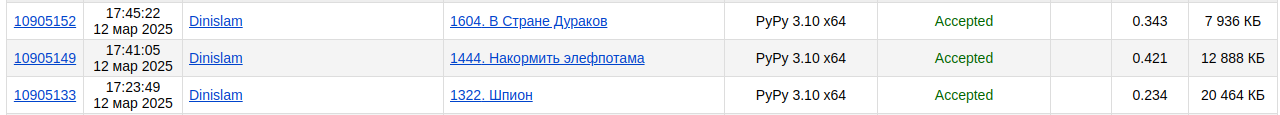
\includegraphics[width=1\textwidth]{check_1.png}
    \caption{Результат проверки}
    \label{fig:compiler-status}
\end{figure}

\end{document}

